\documentclass{anstrans}
\usepackage[acronym, toc]{glossaries}
\newacronym{MIT}{MIT}{the Massachusetts Institute of Technology}
\newacronym{UW}{UW}{University of Wisconsin}
\newacronym{US}{US}{United States}
\newacronym{IAEA}{IAEA}{International Atomic Energy Agency}
\newacronym{SNF}{SNF}{spent nuclear fuel}
\newacronym{HLW}{HLW}{high level waste}
\newacronym{FEHM}{FEHM}{Finite Element Heat and Mass Transfer}
\newacronym{DOE}{DOE}{Department of Energy}
\newacronym{DHS}{DHS}{Department of Homeland Security}
\newacronym{GENIUSv1}{GENIUS}{Global Evaluation of Nuclear Infrastructure 
Utilization Scenarios, Version 1}
\newacronym{GENIUSv2}{GENIUS}{Global Evaluation of Nuclear Infrastructure Utilization Scenarios, Version 2}
\newacronym{CNERG}{CNERG}{Computational Nuclear Engineering Research Group}
\newacronym{GDSM}{GDSM}{Generic Disposal System Model}
\newacronym{GDSE}{GDSE}{Generic Disposal System Environment}
\newacronym{GPAM}{GPAM}{Generic Performance Assessment Model}
\newacronym{FEPs}{FEPs}{Features, Events, and Processes}
\newacronym{EBS}{EBS}{Engineered Barrier System}
\newacronym{EDZ}{EDZ}{Excavation Disturbed Zone}
\newacronym{YMR}{YMR}{Yucca Mountain Repository Site}
\newacronym{EPA}{EPA}{Environmental Protection Agency}
\newacronym{PEI}{PEI}{Peak Environmental Impact}
\newacronym{VISION}{VISION}{the Verifiable Fuel Cycle Simulation Model}
\newacronym{NUWASTE}{NUWASTE}{Nuclear Waste Assessment System for Technical Evaluation}
\newacronym{NWTRB}{NWTRB}{Nuclear Waste Technical Review Board}
\newacronym{OCRWM}{OCRWM}{Office of Civilian Radioactive Waste Management}
\newacronym{UFD}{UFD}{Used Fuel Disposition}
\newacronym{DYMOND}{DYMOND}{Dynamic Model of Nuclear Development }
\newacronym{DANESS}{DANESS}{Dynamic Analysis of Nuclear Energy System Strategies}
\newacronym{CAFCA}{CAFCA}{Code for Advanced Fuel Cycles Assessment }
\newacronym{ORION}{ORION}{O..}
\newacronym{NFCSim}{NFCSim}{Nuclear Fuel Cycle Simulator}
\newacronym{COSI}{COSI}{Commelini-Sicard}
\newacronym{FCT}{FCT}{Fuel Cycle Technology}
\newacronym{SWF}{SWF}{Separations and Waste Forms}
\newacronym{FCO}{FCO}{Fuel Cycle Options}
\newacronym{RDD}{RD\&D}{Research Development and Design}
\newacronym{WIPP}{WIPP}{Waste Isolation Pilot Plant}
\newacronym{ANDRA}{ANDRA}{Agence Nationale pour la gestion des D\'echets RAdioactifs, the French National Agency for Radioactive Waste Management}
\newacronym{TSM}{TSM}{Total System Model}
\newacronym{LANL}{LANL}{Los Alamos National Laboratory}
\newacronym{INL}{INL}{Idaho National Laboratory}
\newacronym{ANL}{ANL}{Argonne National Laboratory}
\newacronym{SNL}{SNL}{Sandia National Laboratory}
\newacronym{LBNL}{LBNL}{Lawrence Berkeley National Laboratory}
\newacronym{LLNL}{LLNL}{Lawrence Livermore National Laboratory}
\newacronym{NAGRA}{NAGRA}{National Cooperative for the Disposal of Radioactive Waste}
\newacronym{CUBIT}{CUBIT}{CUBIT Geometry and Mesh Generation Toolkit}
\newacronym{CSNF}{CSNF}{Commercial Spent Nuclear Fuel}
\newacronym{DSNF}{DSNF}{DOE Spent Nuclear Fuel}
\newacronym{MTHM}{MTHM}{Metric Ton of Heavy Metal}
\newacronym{HTGR}{HTGR}{High Temperature Gas Reactor}
\newacronym{TRISO}{TRISO}{Tristructural Isotropic}
\newacronym{MA}{MA}{Minor Actinide}
\newacronym{CEA}{CEA}{Commissariat a l'Energie Atomique et aux Energies Alternatives}
\newacronym{SKB}{SKB}{Svensk Karnbranslehantering AB}
\newacronym{SINDAG}{SINDA{\textbackslash}G}{Systems Improved Numerical Differencing Analyzer $\backslash$ Gaski}
\newacronym{STC}{STC}{Specific Temperature Change}
\newacronym{LDRD}{LDRD}{Laboratory Directed Research and Development}
\newacronym{LCOE}{LCOE}{Levelized Cost of Electricity}
\newacronym{ABM}{ABM}{Agent-Based Modeling}
\newacronym{COTS}{COTS}{Commercial, Off-The-Shelf}
\newacronym{API}{API}{Application Programming Interface}
\newacronym{RIF}{RIF}{Region-Institution-Facility}
\newacronym{GUI}{GUI}{Graphical User Interface}
\newacronym{HPC}{HPC}{High-Performance Computing}
\newacronym{HTC}{HTC}{High-Throughput Computing}
\newacronym{UML}{UML}{Unified Modeling Language}
\newacronym{MOX}{MOX}{Mixed Oxide}
\newacronym{UOX}{UOX}{Uranium Oxide}
\newacronym{QA}{QA}{Quality Assurance}
\newacronym{NQA1}{NQA-1}{Nuclear Quality Assurance - 1}
\newacronym{VV}{V\&V}{Verification and Validation}
\newacronym{UQ}{UQ}{Uncertainty Quantification}
\newacronym{ASME}{ASME}{American Society of Mechanical Engineers}
\newacronym{NEAMS}{NEAMS}{Nuclear Engineering Advanced Modeling and Simulation}
\newacronym{CI}{CI}{Continuous Integration}
\newacronym{DAG}{DAG}{Directed Acyclic Graph}
\newacronym{XML}{XML}{Extensible Markup Language}
\newacronym{RNG}{RelaxNG}{REgular LAnguage for XML Next Generation}
\newacronym{JSON}{JSON}{JavaScript Object Notation}
\newacronym{SQL}{SQL}{Structured Query Language}
\newacronym{SQLite}{SQLite}{Structured Query Lite}
\newacronym{HDF5}{HDF5}{Hierarchical Data Format version 5}
\newacronym{CSV}{CSV}{Comma-Separated Value}
%\newacronym{<++>}{<++>}{<++>}

\makeglossaries
%%%%%%%%%%%%%%%%%%%%%%%%%%%%%%%%%%%
\title{Cymetric - A Fuel Cycle Metrics Tool for \cyclus}
\author{Anthony Scopatz, Arrielle Opotowsky, Paul P. H. Wilson$^{*}$}

\institute{
$^{*}$Department of Engineering Physics, University of Wisconsin - Madison, 
1500 Engineering Drive, Madison WI 53703
}

\email{scopatz@wisc.edu \and opotowsky@wisc.edu}

%%%% packages and definitions
\usepackage{graphicx} % allows inclusion of graphics
\usepackage{booktabs} % nice rules (thick lines) for tables
\usepackage{microtype} % improves typography for PDF
\usepackage{xspace}
\usepackage{float}
\usepackage{ulem}

\newcommand{\SN}{S$_N$}
\newcommand{\cyclus}{\textsc{Cyclus}\xspace}
\newcommand{\TODO}[1] {{\color{red}\textbf{TODO: #1}}}

%%%% code block stuff
\usepackage{listings}
\usepackage{textcomp}
\usepackage{color}

\definecolor{code}{rgb}{0,0.25,0.25}
\lstset{
    language={Python},
    tabsize=4,
    rulecolor=\color{black},
    upquote=true,
    aboveskip={1.5\baselineskip},
    belowskip={1.5\baselineskip},
    columns=fixed,
    extendedchars=true,
    breaklines=true,
    prebreak=\raisebox{0ex}[0ex][0ex]{\ensuremath{\hookleftarrow}},
    frame=single,
    showtabs=false,
    showspaces=false,
    showstringspaces=false,
    basicstyle=\scriptsize\ttfamily\color{code},
    keywordstyle=\color[rgb]{0,0,1.0},
    commentstyle=\color[rgb]{0.133,0.545,0.133},
    stringstyle=\color[rgb]{0.627,0.126,0.941},
    numberstyle=\color[rgb]{0,1,0},
    identifierstyle=\color{code},
    captionpos=t,
}
\newcommand{\code}[1]{{\color{code}\texttt{#1}}}
    
\begin{document}
%%%%%%%%%%%%%%%%%%%%%%%%%%%%%%%%%%%%%%%%%%%%%%%%%%%%%%%%%%%%%%%%%%%%%%%%%%%%%%%%
\section{Introduction}
Nuclear fuel cycle performance is being given more attention as energy 
experts are attempting to identify a path forward for \gls{US} nuclear power. 
Fuel cycle simulators are of thus of interest because they can provide rapid 
feedback on an array of nuclear fuel cycles. This is generally done by 
computing higher-level aggregate metrics derived from the simulation results. 
Metrics of potential interest to the simulator stakeholders, for example, 
include levelized cost of electricity, proliferation resistance, and various 
quantities and qualities of the \gls{SNF}.

The \cyclus nuclear fuel cycle simulator is a unique approach to the suite of 
existing simulation codes, including many benefits and capabilities.
For example, its modular architecture enables flexible simulations, which 
allows for extensive comparisons at any level of fidelity. Additionally, the 
agent-based modeling approach improves upon traditional system dynamics, adding 
generality to encompass a broad range of simulation cases. \cite{cyclus2015, cyclus_v1.2} 

Simulations are typically evaluated and compared via metrics. This 
prompted the creation of a a new analysis tool, called Cymetric, written for 
\cyclus. When a \cyclus simulation is complete, it stores its information in a 
database. Cymetric can read from and write to a \cyclus database to display 
and/or compute metrics. Cymetric was designed to be easily used, so Python was 
chosen as the interface. Additionally, extensbility and customization of metrics
are a necessity, so Cymetric implements a metric dependency structure easily accessed by a user unfamiliar with the details of \cyclus simulations.

This paper outlines the design and implementation of Cymetric. First described 
is how Cymetric is designed to efficiently interact with a \cyclus database to 
return tables of metrics. Also covered in this section is the dependecy structure of the metrics. 
Next, the two implementations of Cymetric via a command line utility, \code{cymetric},
and a Python interface are detailed.  Within this discussion, it is shown how users can easily 
add their own custom metrics of interest if they are not already included in the
tool. 

%%%%%%%%%%%%%%%%%%%%%%%%%%%%%%%%%%%%%%%%%%%%%%%%%%%%%%%%%%%%%%%%%%%%%%%%%%%%%%%%
\section{Design}
Cymetric was designed with usability and extensibility in mind. 
Cymetric reads in data from a \cyclus{}-generated database. This can be as 
simple as reading in a root table, which is a table included in the \cyclus 
database by default. Or, the request could be for a metric not in the database.
If it is not in the database, it will compute the metric and 
write it back to the database as a table to allow for future retrieval. 

The metrics can be dependent on root tables or other metrics in the
\cyclus database. This dependency system and database writing allows sets of 
related metrics to be computed efficiently. Because metrics are dependent 
on other metrics or root tables, they must form a directed 
acyclic graph (DAG). That is, no circular dependencies are allowed.

For example, one might be interested in the decay heat 
of a batch of \gls{SNF}. The decay heat is calculated using the activity of 
individual nuclides. The activity is calculated from the mass of each nuclide.
This is in turn computed from two root metics generated by 
\cyclus itself: quantity of material (mass) and the mass fraction of each 
nuclide in that material. 
This is depicted graphically in Figure \ref{fig:metdeps}. In this example, 
if the activity was previously calculated for another purpose, it is stored in the database and the additional step of 
determining the decay heat will be less expensive. 

\begin{figure}[htbp!]
\begin{center}
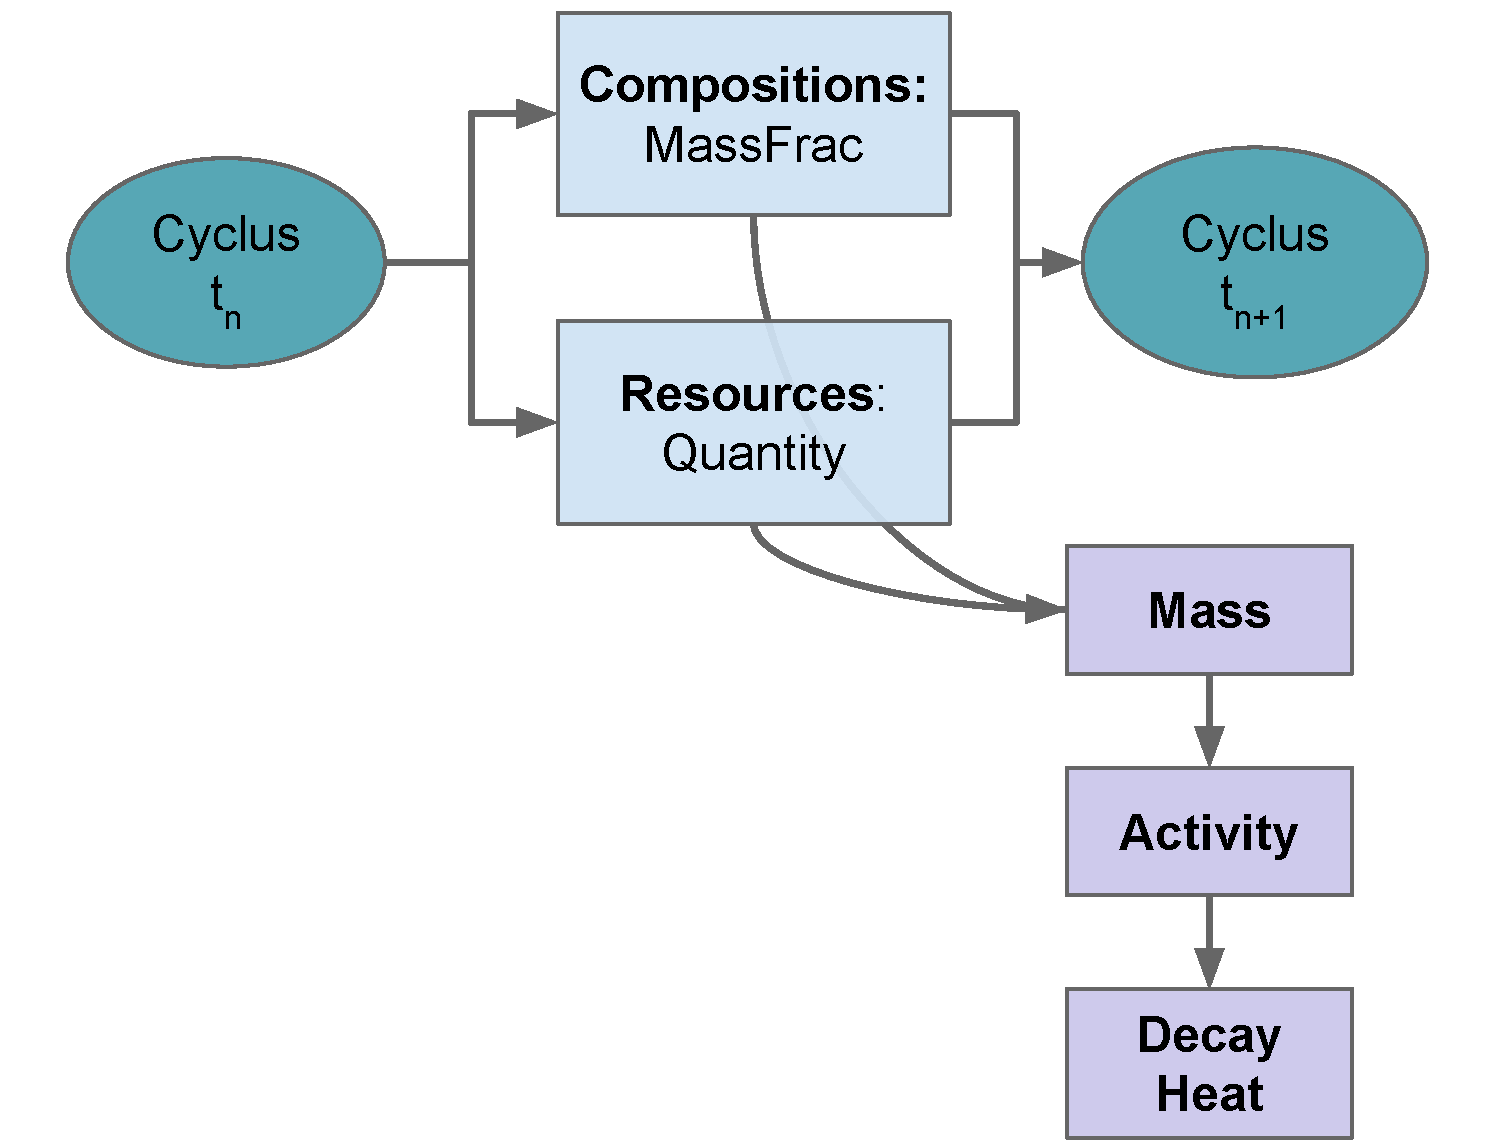
\includegraphics[width=0.5\textwidth]{deps.pdf}
\end{center}
\caption{Metrics can be dependent on root tables and/or other metrics.
         Metrics can be compute per time step (as shown here) or aggregated
         over the entire life cycle of the simulation.}
\label{fig:metdeps}
\end{figure}

%%%%%%%%%%%%%%%%%%%%%%%%%%%%%%%%%%%%%%%%%%%%%%%%%%%%%%%%%%%%%%%%%%%%%%%%%%%%%%%%
\section{Implementation}

There are three main ways that users will interact with cymetric: 
via the command line, via the Python interface, and by writing metrics 
themselves.

\subsection{Cymetric via the Command Line}
The simplest way to become familiarized with the functionality of Cymetric 
is through the command line utility \code{cymetric}. 

The first argument given to this tool is the database of interest. 
Currently, \cyclus supports \gls{HDF5} \cite{folk2011overview} and \gls{SQLite} \cite{owens2006definitive} databases, 
so Cymetric supports both as well. For the purposes of this paper, 
\code{test.sqlite} will be used as the representative cyclus output file. 
The second 
argument given is an optional flag. Either \code{-l} may be provided to obtain 
a listing of the tables currently in the database or the \code{-e} flag 
can be given to execute arbitrary code on a metric. 

A table listing using \code{-l} will print the \cyclus generated tables 
as well as the metadata \cyclus stores. This can be seen in Listing 
\ref{dashl}. After a metric is computed, it shows up on the table 
listing here as well. 

\begin{lstlisting}[caption ={List of Tables in a Database}, label=dashl]
$ cymetric test.sqlite -l
AgentEntry
AgentStateAgent
AgentStateInventories
AgentState_agents_NullInstInfo
AgentState_agents_NullRegionInfo
AgentState_cycamore_BatchReactorCommodPrefs
AgentState_cycamore_BatchReactorInfo
AgentState_cycamore_BatchReactorInitialInv
AgentState_cycamore_BatchReactorRecipeChanges
AgentState_cycamore_EnrichmentFacilityInfo
Compositions
DecayMode
Enrichments
FieldTypes
Finish
Info
InputFiles
MapIntDouble
MapIntInt
MapIntStr
MapStrDouble
MapStrInt
MapStrStr
MaterialInfo
NextIds
Prototypes
Recipes
ResCreators
Resources
Snapshots
Transactions
VectorDbl
VectorInt
VectorStr
XMLPPInfo
...
\end{lstlisting} 
%stopzone

The code execution using \code{-e} is accomplished by including 
Python code in quotes after the flag, as shown in Listing \ref{dashe}. 

\begin{lstlisting}[caption ={Executing Code on a Database}, label=dashe]
$ cymetric test.sqlite -e "<PYTHON CODE HERE>"
\end{lstlisting} 
%stopzone

When a metric or root table is used by Cymetric, it returns the table 
as a pandas DataFrame. \cite{pandas0.15.2} If the table Resources was of interest, 
then one enters \code{print(Resources[:])} inside the quotation marks. 
This outputs the table, a portion of which is shown below in Listing 
\ref{resources}. The full metric is returned if given \code{[:]}, 
\code{[None]}, or \code{[...]}. 

\begin{lstlisting}[caption={Printing a Root Table}, label=resources]
$ cymetric test.sqlite -e "print(Resources[:])"

         SimId   ResourceId  ObjId      Type  
 0    8afed46a...         5      4  Material   
 1    8afed46a...        10      8  Material   
 2    8afed46a...        11      4  Material   
 3    8afed46a...        13      4  Material   
 4    8afed46a...        14      9  Material   
 5    8afed46a...        16      4  Material   
...

  TimeCreated  Quantity Units  QualId  Parent1  Parent2  
0           0  0.00e+00    kg       3        0        0  
1           0  3.14e+05    kg       3        0        0  
2           0  3.14e+05    kg       9        5       10  
3           0  2.36e+05    kg       9       11        0  
4           0  7.87e+04    kg       9       11        0  
5           0  1.57e+05    kg       9       13        0  
...

[224 rows x 10 columns]
\end{lstlisting}
%stopzone

Additionally, the metrics can be filtered direcly from this interface.
Condition filters on column names can be applied. Multiple condition
filters may be separated by commas. For example, if only the plutonium 
isotopes are desired, they can be isolated as shown in Listing \ref{pu}. 

\begin{lstlisting}[caption ={Filtering a Root Table}, label=pu]
$ cymetric test.sqlite \
  -e "print(Compositions[NucId >= 940000000, 
                         NucId < 950000000])"
      SimId     QualId      NucId  MassFrac
0  62079c87...       5  942380000  0.000269
1  62079c87...       5  942390000  0.005667
2  62079c87...       5  942400000  0.002204
3  62079c87...       5  942410000  0.001944
4  62079c87...       5  942420000  0.000820

[5 rows x 4 columns]
\end{lstlisting}
%stopzone

In addition to filters on root tables, metrics can  be calculated directly 
on the command line. A predefined metric, \code{Materials}, can be called 
to calculate the mass of each nuclide for each transaction made during 
the simulation. Furthermore, all operations that are possible in Python 
with pandas DataFrames are also possible on metrics.  This enables the user
to perform run time data manipulation without the need to create a metric.
For example, if the masses are in [g] yet [kg] is needed, 
a conversion factor can be applied as shown in Listing \ref{mass}.

\begin{lstlisting}[caption ={Calculating and Manipulating Metrics}, label=mass]
$ cymetric test.sqlite \
  -e "mass = Materials[:]['Mass'] / 1000; print(mass)"
0      0.711000
1     99.289000
2      0.710954
3     99.282530
4      0.000046
5      0.006470
6      0.710907
7     99.276059
8      0.000046
9      0.006470
10     0.710827
11    99.264806
12     0.000081
13     0.011254
14     0.710790
...
Name: Mass, Length: 209, dtype: float64
\end{lstlisting}
%stopzone

To assist more than just printing tables, there are a number of Python 
modules available when using the execution flag. These are listed below 
in Table \ref{tab:modules} with their aliases.

\begin{table}[htb]
\centering
\caption{Modules Available via Cymetric Command Line Code Execution.}
\begin{tabular}{ll}
\toprule
  Module                   & Alias \\
\midrule
  \code{cymetric}          & \code {cym} \\
  \code{numpy}             & \code{np} \\  
  \code{pandas}            & \code{pd} \\
  \code{uuid}              & \code{uuid} \\
  \code{matplotlib}        & \code{matplotlib} \\
  \code{matplotlib.pyplot} & \code{plt} \\
\bottomrule
\end{tabular}
  \label{tab:modules}
\end{table}

\TODO{Get a pretty graph using matplotlib}

\subsection{Cymetric via Python}
Cymetric provides a full Python interface in addition to the command line 
interface seen above. This grants programatic capabilities to metric 
calculation and derivation. In fact, the command line interface is a thin
wrapper around the functionality provided in the Python interface.
For consistency, it is recommended that users adopt the same the module name 
aliases seen in Table \ref{tab:modules}. 
Table \ref{tab:pyfunc} describes the fucntionality provided by key 
portions of the Python interface.

\begin{table}[htb]
\centering
\caption{Cymetric capabilities provided as Python functions.}
\begin{tabular}{ll}
\toprule
  Function           & Interface                 \\
\midrule 
  \code{dbopen()}    & \code{dbopen(`db')}         \\
  \code{eval()}      & \code{eval(`Metric', db)}   \\
  \code{exec\_code()} & \code{exec\_code(``<PYTHON CODE>'', db)}  \\ 
  \code{root\_metric()} & \code{root\_metric(name=`CustomTable')}  \\
\bottomrule
\end{tabular}
\label{tab:pyfunc}
\end{table} 

An example of an implementation of the above functions is shown below in 
Listing \ref{funcs}. The database is opened via \code{dbopen()}. The 
function \code{eval()} evaluates and reads a metric or root table from the 
database. It allows for filtering conditions to be provided by a list of 
3-tuples of strings. 
Lastly, \code{exec\_code()} provides the same functionality as the
\code{cymetric} command line utility if one desures to incrementally contruct Cymetric code. This could be advantageous for a possible future *.cym file format.

\begin{lstlisting}[caption ={Example Python Script Using Cymetric}, label=funcs]
import cymetric as cym

db = cym.dbopen('test.sqlite')

# print 
evaler = cym.Evaluator(db)
frame = evaler.eval('Materials', db, 
                    conds=[('NucId', '==', 922350000)])
print(frame)

# accomplishes the same output as above
cym.exec_code("print(Materials[NucId == 922350000])", 
              db)
\end{lstlisting}

In Listing \ref{funcs}, an \code{Evaluator} object was created. 
Creating an object in this way and calling its \code{eval()} method directly 
is the most efficient way to evaluate metrics. This is because
it prevents excessively reading from the database.

Lastly, \cyclus allows for the creation of custom tables, and these are not accessible in Cymetric in the same way as the default root tables. These custom tables can be retrieved via the \code{root\_metric()} function shown in Table \ref{tab:pyfunc}.

\subsection{Writing Metrics in Cymetric}
The richness of Cymetric will come largely from its suite of metrics. 
That this suite is extensible by any user at any time will be a major 
factor in its success. For example, radiotoxicity from \gls{SNF} can 
be calculated in many different ways. Sieverts per generated electricity 
or Sieverts per metric ton of uranium or \gls{SNF} are typically used to 
quantify this value. Further complicating this metric, the doses are determined differently, as 
ingestion dose rates or total effective equivalent doses may be used. 
Since the Cymetric developers cannot predict all relevant scenarios, 
user-driven extensibility was built into Cymetric from the ground up. 

Currently, a metric must be written with a function that accepts a pandas 
series and returns a pandas DataFrame. Metrics are defined via the
\code{$@$metric()} decorator, which takes three arguments: the name of the 
metric, its dependencies, and the schema of the metric. 
The name is given as a string. The dependencies are a list of 3-entry tuples. 
Each one includes the name of the table, a tuple column names that are to 
index the series, and the column that is the value of the series. 
The metric schema provides the structure of the metric table and is a 
list of 2-entry tuples: the column name followed by its \cyclus datatype. 
A simple example is depicted below in Listing \ref{massmetric}. This metric 
is only dependent on the column \code{Mass} from the \code{Materials} metric. 

\begin{lstlisting}[caption ={Writing a Metric in Cymetric}, label=massmetric]
deps = [('Materials', ('SimId', 'ResourceId', 'NucId'), 
         'Mass')]

schema = [('SimId', cym.UUID), 
          ('ResourceId', cym.INT),
          ('NucId', cym.INT),  
          ('MassSquared', cym.DOUBLE)]

@cym.metric(name='MaterialsSquared', depends=deps, 
            schema=schema)
def mats_sqrd(series):
    mats = series[0]
    rtn = mats**2
    rtn.name = 'MaterialsSquared'
    rtn = rtn.reset_index()
    return rtn
\end{lstlisting}


%%%%%%%%%%%%%%%%%%%%%%%%%%%%%%%%%%%%%%%%%%%%%%%%%%%%%%%%%%%%%%%%%%%%%%%%%%%%%%%%
\section{Conclusions}

Cymetric is an efficient and extensible tool with which to compute fuel cycle metrics from a \cyclus simulation. It works directly with a \cyclus database and stores metrics as a table in the database itself. It is designed to be easily accessible via Python, and is customizable with user-input metrics. Future work will involve an expansion of the suite of metrics within Cymetric, as well as integration with the \cyclus \gls{GUI}. 

\section{Acknowledgments}
This work has been funded by the \gls{DOE} Nuclear Energy University Program and the \gls{DHS} Nuclear Forensics Graduate Research Fellowship Program. 

%%%%%%%%%%%%%%%%%%%%%%%%%%%%%%%%%%%%%%%%%%%%%%%%%%%%%%%%%%%%%%%%%%%%%%%%%%%%%%%%
\bibliographystyle{ans}
\bibliography{cymetric}
\end{document}
